\documentclass[11pt]{amsart}
\usepackage{graphicx,xspace}
\usepackage{fullpage}
\usepackage{hyperref}
\usepackage{amsmath}
\usepackage{amsfonts}
\usepackage{verbatim}


\newenvironment{definition}[1][Definition]{\begin{trivlist}
\item[\hskip \labelsep {\bfseries #1}]}{\end{trivlist}}


\title{ADAM:  Analysis of Discrete Models of Biological
Systems Using Computer Algebra}
\author{Franziska Hinkelmann$^{a,b}$,
Madison Brandon$^{c,*}$,
Bonny Guang$^{d,*}$,\\
Rustin McNeill$^{e,*}$,
Alan Veliz-Cuba$^{a,b}$, Grigoriy Blekherman$^{a}$, Reinhard Laubenbacher$^{a,b}$}

\begin{document}
\maketitle
{\footnotesize
     \centerline{$^a$Virginia Bioinformatics Institute, Blacksburg, VA 24061-0123, USA}
}

{\footnotesize
  % please put the address of the second  and third author
     \centerline{$^b$Department of Mathematics,
      Virginia Polytechnic Institute and State University, Blacksburg, VA 24061-0123, USA}
}

{\footnotesize
  % please put the address of the second  and third author
     \centerline{$^c$University of Tennessee - Knoxville, Knoxville, TN 37996-2513, USA}
}

{\footnotesize
  % please put the address of the second  and third author
     \centerline{$^d$Harvey Mudd College, Claremont, CA 91711-5901, USA}
}


{\footnotesize
  % please put the address of the second  and third author
     \centerline{$^e$University of North Carolina - Greensboro, Greensboro, NC 27402-6170, USA}
}

%%  Q: Is this what Reinhard wanted?
%%  A: Well gosh, why don't you ask him -Bonny
{\footnotesize
     \centerline{$^*$These authors contributed equally}
}

%\date{20 July 2010}


\begin{abstract}

Many biological systems are modeled qualitatively with discrete models, such as 
probabilistic Boolean networks, logical models, bounded petri-nets, and agent-based models.
Simulation is a common practice for analyzing discrete models, but many systems are far too large
to capture all the relevant dynamical features through simulation alone. We convert discrete models into algebraic models
and apply tools from computational algebra to analyze the dynamics of discrete systems. 
\begin{comment}
We use various abstract algebra techniques to
develop algorithms and software to analyze discrete models for key dynamic
features of biological relevance.
\end{comment}
The key feature of biological systems that is exploited by our algorithms is their sparsity: while the number of genes (or agents) in a
biological network may be quite large, each gene is affected only by a small number of other genes. This allows for fast Gr\"{o}bner basis 
computations in the algebraic models.
All algorithms and methods are available in our package  Analysis of Discrete Algebraic Models (ADAM), are available through a 'modeler friendly' web-interface
that allows for fast analysis of large models, without requiring understanding of the underlying mathematics or any software installation.
\begin{comment}
 By providing a user-friendly interface to fast analysis tools, %this sounds weird -B
we promote the use of discrete models to model large complex systems.
\end{comment}
\end{abstract}

\section*{Acknowledgments}
The authors would like to thank Prof Monika Heiner for clarifying the Petri
net terminology.
Funding: REU NSF Fund number 0755322, Army research grant, Alan's
NSF fund, other funds?

% Introduction
% Results, i.e., ADAM,  Application
% definitions and methods
% Discussion

\section{Introduction}
\begin{comment}
% Modeling, Discrete vs continuous models
Mathematical modeling is a crucial tool in understanding the dynamic behavior of
biological systems. Continuous differential equations models are commonly used, but they rely on
the knowledge or estimation of parameter rates, which are often hard to obtain. Discrete models
offer slightly coarser qualitative information, but do not require the fine parameter data to set up.
In many instances the qualitative is already quite interesting and unknown. 
%Discrete models are often very intuitive and easily understood by life
%scientists.
\end{comment}
% Different discrete models and lack of analysis tools
Discrete models are widely used in studying dynamical behavior of biological systems. Model types include
(probabilistic) Boolean networks, logical networks, Petri-nets, Cellular
automata, and Agent-based (individual-based) models. 
However, there is a lack of tools
for analyzing dynamical behavior of large-scale discrete models. Commonly the analysis is performed by simulation, meaning that an
initial configuration of the system is iterated a prescribed number of times, or until a
steady state is found. Since the number of initial configurations grows exponentially in the number of variables, simulation
will not provide a complete picture of dynamical behavior for large models.
Simulation is especially inefficient for non-deterministic
systems, since simulations must be run many times to obtain meaningful
probability estimates.

% Math framework and Groebner basis
All of the  different types of discrete models mentioned above can be converted into the unified framework of polynomial dynamical systems \cite{Alan:Bioinf2010, Hinkelmann:2010}. This allows us to apply tools from computational commutative algebra to analyze their dynamics. We developed an online software package ADAM, Analysis of Discrete Algebraic Models \cite{ADAM}, which automatically converts discrete models into polynomial dynamical
systems, and then analyzes their dynamics by using various computational algebra techniques. Even for large systems, ADAM
computes key dynamic features, such as fixed points, in a matter of seconds.
\begin{comment}
When discrete models are described within a mathematical framework,
mathematical theory and computational tools can be used to analyze them.
Algebraic models have been proposed as
a common framework for discrete models
\cite{Alan:Bioinf2010, Hinkelmann:2010}, which firmly grounds them into
the framework of algebraic geometry and computational algebra. Within this
framework, Gr\"obner basis calculations can be used to analyze complex
networks efficiently.
\end{comment}
%ADAM


\section{Results}
% ADAM available for free, platform independent
We developed a software package {\it Analysis of Dynamical Algebraic Models,
ADAM} \cite{ADAM} which uses a combination of simulation
and computational algebra techniques to analyze discrete models.
ADAM is available online free of charge. It is platform
independent and does not require installation of any software or computer
algebra tool. ADAM is highly suitable to be used in a class room as a first
introduction to discrete models as it does not require the students to run
anything else but a web browser.
%% different input types
ADAM allows the following {\bf inputs}.
\begin{itemize}
  \item Logical models generated with GINsim \cite{GINsim}
  \item Petri-nets generated with Snoopy \cite{Snoopy}
  \item polynomial dynamical systems
  \item Boolean networks
  \item probabilistic networks \cite{shmulevich}.
\end{itemize}
Logical models, Petri-nets, and Boolean networks are automatically converted
into the corresponding polynomial dynamical system as described in
\cite{Alan:Bioinf2010}, so that algorithms from computational
algebra can be used to analyze the dynamics.

% output
We developed and implemented several different algorithms that allow one to analyze
important features of algebraic models when they are too large for pure simulation.
Most algorithms rely on Gr\"obner basis calculations to find key dynamic
features.
Since the polynomials in the algebraic
models originate from biological systems, we can exploit their structural
features to secure very fast Gr\"obner basis computations.
For small enough models, ADAM generates a graph of the complete phase space.
When the phase space is too large to be drawn or when a visualization is not
needed, ADAM generates the following {\bf output}.
\begin{itemize}
  \item a graph of wiring diagram
  \item fixed points (for deterministic and probabilistic systems)
  \item limit cycles of length $m$
  \item trajectories originating from a given initial state until a stable
  attractor is found
  \item dynamics for synchronous or asynchronous updates
  \item functional circuits
  \item a complete description of the phase space for conjunctive/disjunctive
  networks.
\end{itemize}

%explain that everything is a polynomial and how equations relate to dynamics
The key idea behind our algorithms is that discrete models have finitely many states and computations 
can be performed over a finite field \cite{Alan:Bioinf2010,
Hinkelmann:2010}. Since any function over a finite field is a polynomial
\cite{Lidl:1997} we convert discrete models into polynomial dynamical systems
and use commutative algebra algorithms. More specifically, the problem of finding fixed points and limit cycles
can now be reformulated as solving a system of polynomial equations. We use Gr\"{o}bner basis techniques to solve the 
resulting system of polynomial equations. Gr\"obner basis calculation is for polynomial systems what
Gauss-Jordan elimination is for linear systems: a structured way to transform
the original system to triangular shape without changing its solution space.
The triangular shape of the resulting systems allows for stepwise retrieval of  the solutions of the system.



%Once a
%basis in lexicographic monomial order is found, solutions are easily generated
%by back-substitution (see benchmark results \ref{benchmarks}).

% Sparse systems
The efficiency of the Gr\"obner basis calculations is largely dependent on the
assumption that most discrete models arising from biological systems are
sparse, meaning that every variable is only affected by a small subset of the
total variables in the system.  It has been suggested, that in robust gene
regulatory networks genes are regulated by only a handful of regulators
\cite{Leclerc:2008}.  Thus the PDS representing such biological networks are
sparse, i.e., each function depends only on a small subset of the total nodes.

%....Insert heuristic explanation for why we think the GB algorithm is fast on
%sparse systems..
In the worst case, computing Gr\"obner bases for a set of polynomials has a
complexity of doubly exponential in the number of solutions to the system.
However, in practice Gr\"{o}bner bases are computable in a reasonable time, and
for the sparse systems over a finite field that are common in discrete
biological models, it is actually fairly fast. In the first place, computing
Gr\"{o}bner bases in modular form have been shown to be much faster usually
\cite{Brown:1971}. In addition, sparse polynomials mean that simpler
S-polynomials, usually of the same length, will be added, causing the Groebner
basis computation to be easier.
Based on benchmarking tests
for randomly generated systems and 25 logical models of biological systems
\cite{GINsim}, the computations are very fast, and finish on the scale of
seconds.

\section{Application} \label{benchmarks}% This needs more work
For most biological systems, we can assume that the wiring diagram is sparse
\cite{Ting:1999},
i.e., every regulator is influenced by only a handful of other regulators. We
tested ADAM to analyze systems for fixed points on randomly generated
polynomial dynamical systems that have the same sparse structure that we
expect from gene regulatory networks. All calculations ran in a matter of seconds on
a 2.7 GHz computer. In addition, we used ADAM to analyze all logical models
available in the GINSim model repository \cite{GINsim} as of August 2010. These are logical
models of several biological systems, most of which have been published in
peer reviewed journals. ADAM was able to convert 27 out of 29 (? Madison will
find this out) logical
models to polynomial dynamical systems.

Fixed points and limit cycles up to length 20 were computed for all 25 models
with 85 percent of computations finishing in less than a second and
collectively all computations finishing in less than 30 minutes. Networks size
and run time are depicted in Figure \ref{fig:chart}.
\begin{comment}
\begin{figure}[htb]
  \centering
  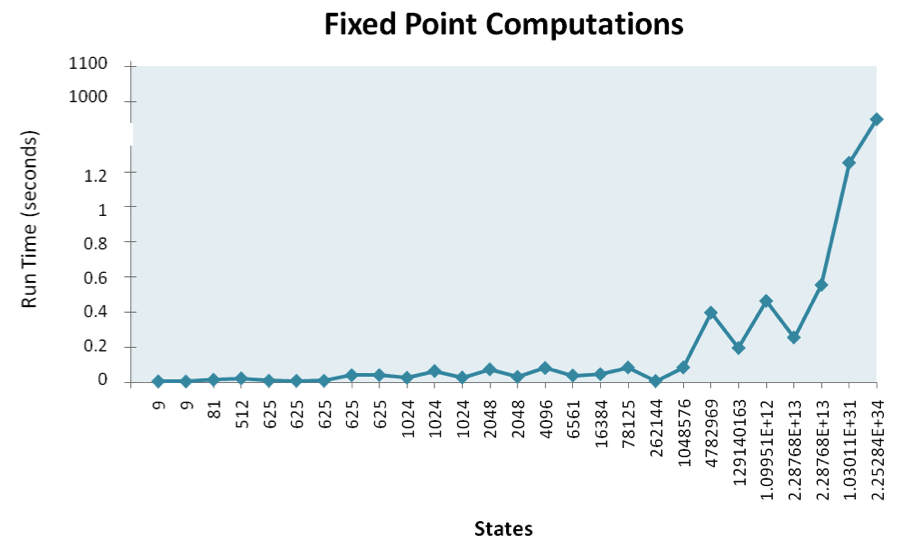
\includegraphics[width=0.95\textwidth]{GINSimChart.png}
  \caption{Runtime of fixed points calculations of several logical models from
  \cite{GINsim}. Executed on a 2.7 GHz computer.}
  \label{fig:chart}
\end{figure}
\end{comment}
We were not
able to analyze this model for fixed points using GINSim, after several hours
it ran out of memory (?).
In addition to theoretical testing, benchmark tests were done on 25 models from the GINsim repository, including two in excess of 50 nodes.  Fixed points and limit cycles up to length 20 were computed for all 25 models with 85 percent of computations finishing in less than a second and collectively all computations finishing in less than 30 minutes.

% Example application
We demonstrate the power of ADAM on a well understood model of the
expression pattern of the segment polarity genes in Drosophila melanogaster
\cite{AO}. The Boolean Model consists of 60 variables. ADAM identifies 10
fixed points as previously found in the publication within a second. ADAM also
quickly computes that there are no limit cycles of length two, an analysis
that was not done previously and which is encouraging since no oscillatory
behavior was observed experimentally. The model file in ADAM format can be accessed at
\cite{??}.



\section{Methods}
For this manuscript to be self contained, we will now go over the definitions
of several discrete models and polynomial dynamical systems.

Discrete modeling approaches have been applied
to a wide variety of biological contexts, including metabolic networks, gene
regulatory networks, tumor growth, population models, radiation therapy
\cite{Richard}, and signal transduction networks.
It has been shown that any set of functions describing a discrete model can be
written as a system of polynomial equations or a polynomial dynamical system
(PDS) in a finite field \cite{Lidl:1997}.
There are several types of discrete models including Logical models, Petri
Nets, and Agent-Based models, all of these can be translated into polynomial
dynamical systems \cite{Alan:Bioinf2010,Hinkelmann:2010}.

\subsection{Polynomial Dynamical System (PDS)}
\begin{definition}{Polynomial Dynamical Systems \cite{JLSS}}
A polynomial dynamical system (PDS) over a finite field $k$ is a function
$$f = (f_1, \ldots, f_n) : k^n \rightarrow k^n,$$
with the coordinate functions $f_i \in k[x_1, \ldots , x_n]$. Iteration of $f$ results
in a time-discrete dynamical system. PDSs are special cases of finite
dynamical systems, which are maps $X^n \rightarrow   X^n$ over arbitrary
finite sets $X$.
\end{definition}


\begin{definition}{Probabilistic Polynomial Dynamical Systems}
A probabilistic networks over a finite field $k$ is a function
$$f = (\{f_{1,1}, \ldots, f_{1, r_1}\}, \ldots, \{f_{n, 1}, \ldots, f_{n, r_n}
\}) : k^n \rightarrow k^n,$$
with the coordinate functions $f_i \in k[x_1, \ldots , x_n]$ and $n$
distribution functions $\Gamma_i$ that assign a probability $p_{i,j}$ to each
$f_{i,j}$. $\sum_{j=1} ^ {r_i} p_{i,j} = 1$ for all $i \in \{1, \ldots, n\}$.
\end{definition}
This means at every iteration, for each variable $x_i$ one of the functions in
$\{f_{i,1}, \ldots, f_{i, r_i}\}$ is randomly chosen to update $x_i$.
Specifically, probabilistic Boolean networks (PBN) have been studied
extensively \cite{shmulevich}.

ADAM accepts PBN as input. It can simulate the
complete state space for small enough models, by generating every possible
transition and labeling the edge with its probability according to the
distribution. If no distribution is given, ADAM assumes a uniform distribution
on all functions. For large networks, ADAM's {\it Algorithm} choice computes fixed points of probabilistic networks, but no limit cycles.

\subsubsection{Key Dynamic Features}
Polynomial dynamical systems have several dynamic features with biological
relevance. These include the number of components, component sizes, fixed
points, limit cycles, and limit cycle lengths.

For the purpose of simplifying our explanations, we will focus on a Boolean
Network example. Consider the state space of the following three node Boolean
Network $f:\mathbb F_2^3 \rightarrow \mathbb F_2^3$
\begin{align}
f1 &= x1*x2*x3+x1*x2+x2*x3+x2\notag \\
f2 &= x1*x2*x3+x1*x2+x1*x3+x2+x1 \notag \\
f3 &= x1*x2*x3+x2*x3+x1*x3+x2+x1. \label{equ:example}
\end{align}
The wiring diagram showing the static interaction of the three variables is
depicted in Figure \ref{fig:WD} along with its phase space in Figure ~\ref{fig:SS}.
The phase space shows how the network is dynamically evolving. Each state is
represented by a vector of three entries, variable 1, 2, and 3. Arrows
indicate how a state is changing as the update function is applied. Example
\ref{equ:example} has one fixed points, $(0,0,0)$ and a limit cycle of length
three, $(0,1,0) \rightarrow (1,1,1) \rightarrow (0,1,1) \rightarrow (1,1,1)$.
Fixed points correspond to steady states of the biological systems. Limit
cycles indicate recurring processes in the system, for example different
stages of the cell cycle.

\begin{comment}
\begin{figure}[ht]
\begin{minipage}[here]{0.5\linewidth}
  \centering
  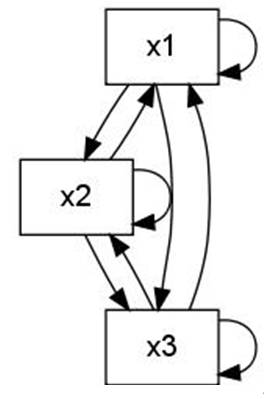
\includegraphics[scale=0.55]{exampleWD.jpg}
  \caption{Example wiring diagram with 3 nodes}
  \label{fig:WD}\end{minipage}
\hspace{0.5cm}
\begin{minipage}[here]{0.5\linewidth}
  \centering
  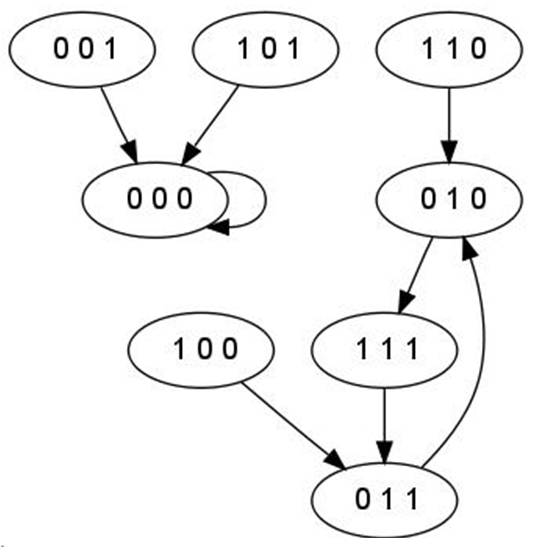
\includegraphics[scale=0.55]{exampleSS.jpg}
  \caption{Example state space with 3 nodes and two possible states per node, 0 or 1, hence $2^3=8$ states}
  \label{fig:SS}
\end{minipage}
\end{figure}
\end{comment}
%\begin{figure}[here]
%	\centering
%	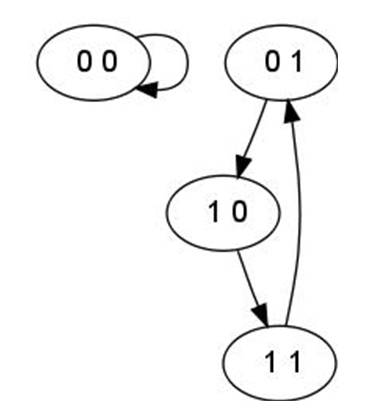
\includegraphics[scale=0.75]{2by2Ex_statespace.jpg}
%	\caption{Example State space of a simple two node Boolean Network}
%	\label{fig:2by2Ex}
%\end{figure}

\subsection{Logical Models and Petri Nets}
ADAM can automatically convert logical models and $k$-bounded petri nets to
polynomial dynamical systems \cite{Alan:Bioinf2010}. In order to be understood
by ADAM, logical models must be
generated with GINSim \cite{GINsim} and petri nets with Snoopy \cite{Snoopy}.
We are planning to implement conversion for agent-based models as described in
\cite{Hinkelmann:2010}.

\subsubsection{Functional Edges}
ADAM will also identify functional circuits and their sign, as defined in \cite{Chaouiya}.
An edge is called functional, if {\bf This definition is not correct ( edge. Let $x = (x_1, x_2, \ldots, x_n) \in \mathbb{F}^n_p, p$ prime and let $f_i$ be a function on $x$. A functional edge $j \rightarrow i$ is one such that
$f_i(x_j = a) \neq f_i(x_j = b)$ for some $a \neq b \in \mathbb{F}_p, x_j \in
x$. ) }
In other words, an edge from $i$ to $j$ is functional, if there is at least
one state, such that changing only $x_i$ but keeping all other values fixed,
changes the state of $f_j$.

Now, given a functional edge $j \rightarrow i$, it is signed positive if $f_i(x_j = a) \leq f_i(x_j = b)$ for all $a < b, x_{q \neq j}$ constant. In other words, $j \rightarrow i$ is positive if increasing $x_j$ while keeping all other $x_q \in x$ constant causes $f_i$ to either increase or stay equal.

Likewise, $j \rightarrow i$ is signed negative if $f_i(x_j = a) \geq f_i(x_j = b)$ for all $a < b, x_{q \neq j}$ constant. A functional edge does not have a sign otherwise.

As an example, suppose we have $x = (x_1, x_2) \in \mathbb{F}^2_2$. Let $f_i(x) = x_1+x_2+x_1*x_2$. We want the sign of $1 \rightarrow i$. When $x_2 = 0$, we see that
\[ f_i(x_1 = 0) = 0 \leq f_i(x_1 = 1) = 1, \]
and when $x_2 = 1$, we see that
\[ f_i(x_1 = 0) = 1 \leq f_i(x_1 = 1) = 1, \]
hence $1 \rightarrow i$ is a positive edge.

Identifying functional edges is useful because it informs the modeler which genes actually have an effect on another gene's state. In ADAM, all edges drawn in the dependency graph are functional.  Identifying the sign of an edge has two uses. First, it informs the modeler about how a gene affects another gene - whether it activates or inhibits the gene. Second, the product of the signs of edges in a circuit determines the sign of the circuit. It has been shown that the existence of more than one fixed point and other dynamics relies on the number and the sign of functional circuits in a dependency graph \cite{Thomas:2001}\cite{Remy:2005}.


\subsection{Conjunctive/Disjunctive Networks}
There are some classes of functions which have a certain structure that can be
exploited to achieve faster calculations.  For example in \cite{conjunctive} it is shown that when input functions are of the class of Conjunctive or Disjunctive Boolean Networks then key dynamic features can be found with almost no computational effort.  Conjunctive Boolean networks consist of functions containing only one monomial term, i.e. the functions use only the AND operator.  Conversely, Disjunctive Boolean Networks consist of functions which use only the OR operator.  We include a separate algorithm to compute dynamics in the case of Conjunctive/Disjunctive Boolean Networks.  Currently this option only works on strongly connected graphs.


Our algorithms were coded in the software system Macaulay2 \cite{Macaulay2}.  Macaulay2 is a computer algebra system that incorporates ideas from abstract algebra.  Specifically we used Macaulay2 to compute the Gr\"obner basis of input functions within a specified ring.  We implemented the Gr\"obner basis algorithm with the `Sugarless' option which, after running benchmark tests, we found to be faster with our systems.

In the worst case, computing Gr\"obner bases for a polynomial system has a
complexity of doubly exponential in the number of solutions to the system.
However, in practice Gr\"obner bases are computable in a reasonable time.
Furthermore, for sparse systems in a finite field it is actually fairly quick.
It has been shown that computing Gr\"obner bases in modular form is much
faster in general. \cite{Brown:1971} In addition, sparse polynomials mean that
simpler S-polynomials, usually of comparable length, will be added to the
basis, which means less computation is involved.  In short, the sparse
structure of biological systems is preserved by Gr\"obner bases, causing our
algorithms to be both efficient and fast. See the Applications section for
benchmark tests results for Gr\"obner bases computations.

The algorithms to compute dynamics for Conjunctive/Disjunctive Networks can be
found in Jarrah et al. \cite{Alan:Bioinf2010}, and were also coded in Macaulay2.

\subsection{Analysis of stable attractors}
Every attractor in a deterministic polynomial dynamical systems is either a
fixed points or a limit cycles. ADAM can analyze large models for fixed points
and limit cycles of a given length.

Fixed points of a polynomial dynamical system $f$ must satisfy the equation $f(x)
= x$, as no coordinate of $x$ is changing as it is updated. Similarly, states of a
limit cycle of length $m$ satisfy the equation $f^m(x) = x$. ADAM computes all
fixed points by solving the system $f_i(x) - x_i = 0$ over $\mathbb F_p^n$ for $i \in \{1, \ldots,
n\}$, where $p$ is the characteristic of the final field. First, a Gr\"obner
basis in lexicographic order is computed. The elements of the basis are in
triangular form, meaning that the first equations involved the smallest number
of variables, and the last equations the most. This allows to solve the system
by back substitution instead of enumeration all $p^n$ points in $\mathbb
F^n_p$ and testing whether they are solutions.
All calculation are implemented in Macaulay2 \cite{Macaulay2}, a
computer algebra system.

For limit cycles of length $m$, the solutions of $f^m(x)=x$ are found and then
grouped into cycles, by applying $f$ to each of the solutions.
%  begin GINsim discussion
% Should parts of this be moved to 2.1?
%In addition to inputting a list of functions to our software, the user also
%has the option of uploading a GINsim file for analysis \cite{GINsim}.  GINsim
%is an online computer tool used to construct models of gene networks.  The
%model is formed with a set of nodes, a set of edges, the level of
%concentration or expression of the nodes, and a set of parameters. GINsim
%creates a file containing the information of the biological system and this
%file can be uploaded to our software. When input is a GINsim file, the file
%is first converted to a PDS \cite{Alan:Bioinf2010}, and is then analyzed in the same manner discussed above for fixed points and limit cycles of specified length.


\section{Conclusion}

Discrete Modeling techniques are a useful tool for analyzing biological
systems. Upon translating a discrete model, such as logical networks,
petri-nets, or agent-based models into an algebraic model, rich mathematical
theory becomes available. This enables one to
avoid simulation which is limited because of combinatorial explosion. The algorithms
we developed are fast for sparse systems, a structure maintained by most biological
systems. All algorithms have been included in the software package ADAM\cite{ADAM},
which is user-friendly and available as a free web service.
We hope to expand ADAM to an all-encompassing Discrete Toolkit which incorporates more
analytical methods, better visualization, and automatic conversion for more model types.
We also hope to analyze controlled algebraic models and expand theory to stochastic systems.

\appendix
\section{Paragraphs I removed from main section}
To demonstrate how this process works consider the Lambda Phage model from
earlier, this time modeled with four genes: Cro, CI, CII, and N. The model of
lysogenization in the Lambda Phage is available from the model repository on the GINsim website. (see Figure ~\ref{fig:phageWD})
Lambda phage is a virus which hijacks a host cell by injecting its DNA into
the host and assuming replication processes in order to produce more phage
particles.  There are two phases of viral reproduction, the lytic cycle and
the lysogenic cycle.  In the lysogenic cycle, the phage integrates itself into
the host cell's genome.  At this point the phage DNA is called a prophage.
Whenever the host cell divides, the prophage is duplicated.  When the host
cell comes under stress the new DNA is released causing proliferation of new
phages.  Specifically, in the Lambda Phage, this cycle occurs when CII reaches
a high enough concentration to activate certain promoters.  One of these
promoters produces an antisense which reduces Cro production, represented in
the wiring diagram by the red arrow from CII to Cro which means that CII
inhibits Cro.  This promoter also turns on the CI gene which acts as a
repressor to the other genes.  At this point the phage DNA is integrated into
the host's chromosome.  The repression of the other genes by CI maintains the
concentration of CI in the system.  In fact, lysogeny is maintained solely by
CI.  CI controls its own expression, as can be seen in the wiring diagram from
the green arrow which loops from CI back to itself, and it remains present
throughout the lysogenic cycle.

%%% I got this info from wikipedia.  should i cite it? I feel like it might be dumb to cite wiki..


\begin{comment}
\begin{figure}[h]
	\centering
	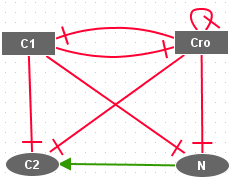
\includegraphics[scale=0.84]{PHAGE4nice.png}
	\caption{Wiring Diagram of lysoseginiation by Lambda Phage}
	\label{fig:phageWD}
\end{figure}
\end{comment}
When the file is uploaded to our software, the following polynomial dynamical system is returned:\\
\begin{align}
f1 &= -2x_{2}^{4}+2 \\
f2 &= x_{1}^{4}x_{2}^{4}+x_{1}^{4}x_{2}^{3}-2x_{1}^{3}x_{2}^{4}-2x_{1}^{3}x_{2}^{3}-2x_{1}^{2}x_{2}^{4}-2x_{1}^{4}x_{2}-2x_{1}^{2}x_{2}^3 -2x_{1}x_{2}^{4}-x_{1}^{4}-x_{1}^{3}x_{2}-2x_{1}x_{2}^{3}+2x_{2}^{4}+2x_{1}^{3}-x_{1}^{2}x_{2}+2x_{2}^{3}+2x_{1}^{2}-x_{1}x_{2}+2x_{1}+x_{2}-2 \\
f3 &= 2x_{1}^{4}x_{2}^{4}x_{4}^{4} + x_{1}^{3}x_{2}^{4}x_{4}^{4}+x_{1}^{2}x_{2}^{4}x_{4}^{4}+x_{1}x_{2}^{4}x_{4}^{4}- 2x_{1}^{4}x_{4}^{4}
-x_{2}^{4}x_{4}^{4}-x_{1}^{3}x_{4}^{4}-x_{1}^{2}x_{4}^{4}-x_{1}x_{4}^{4}+x_{4}^{4}\\
f4 &= 2x_{1}^{4}x_{2}^{4}+x_{1}^{4}x_{2}^{3}+x_{1}^{4}x_{2}^{2}+x_{1}^{4}x_{2}-x_{1}^{4}-2x_{2}^{4}-x_{2}^{3}-x_{2}^{2}-x_{2}+1
\end{align}
Analysis is then performed on this system of equations.  ADAM displays the dynamics along with the PDS representing the system. (see Figure ~\ref{fig:ADAMoutput})
\begin{comment}
\begin{figure}[h]
	\centering
	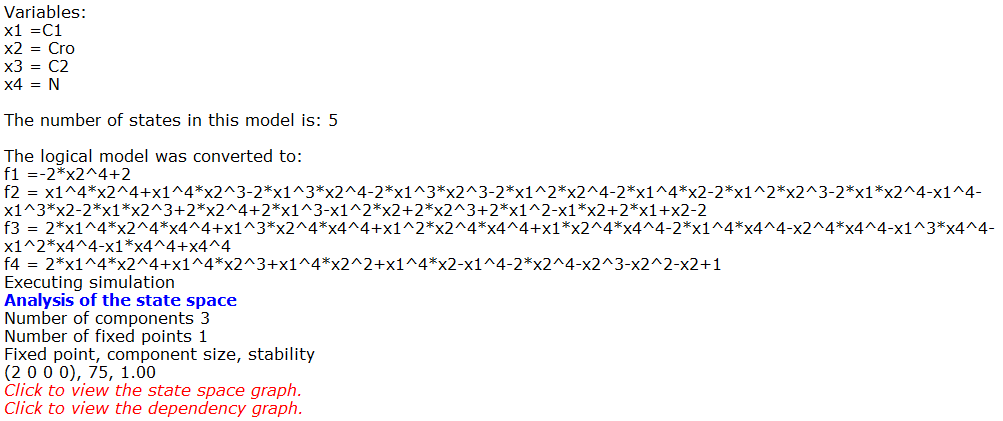
\includegraphics[scale=0.6]{phage4output.png}
	\caption{Example output from ADAM}
	\label{fig:ADAMoutput}
\end{figure}
\end{comment}




However, attempting to find limit cycles using the Gr\"obner basis results in dense polynomial equations. This is because finding limit cycles depends on repeated compositions of the polynomial functions.
%% Is this part in the wrong section?  I dunno.
For instance, solving a system for fixed points equates to solving the system:
\begin{center} \begin{align} f_1-x_1 &=0 \\ \cdots \\ f_n-x_n &=0 \end{align} \end{center}
Whereas finding a limit cycle of length $2$ equates to solving the system:
\begin{center}
  \begin{align}
    (f_1)^2 - x_1 &=0 \\ \cdots \\ (f_n)^2 - x_n &=0
  \end{align}
\end{center}
Even with just one composition, a given node depends not only on its neighbors, but also the neighbors of its neighbors.  Hence the sparse structure of the PDS is lost with repeated compositions. For this reason, our default setting only looks for limit cycles up to length 5 for large networks (those with 10 or more nodes).  The user may also specify a limit cycle length to search for, but should keep in mind that it may take a long time to compute depending on the complexity of the system.  Additional options to the Gr\"obner basis algorithm in Macaulay2 such as $"$Long Polynomial$"$ may aid in the computation of dense systems of equations.

\section{}
It has been shown that in biological systems, input generally only comes from
a few nodes per node.  For instance, in gene regulatory networks genes are
regulated by only a handful of regulators, usually less than 10.
\cite{Ting:1999}  Thus the PDS representing such biological networks are
sparse, i.e. each function depends only on a small subset of the total nodes.
Based on benchmark tests on the algorithms which use Gr\"obner basis to
compute fixed points, we claim that the algorithms are particularly fast on large sparse systems. (see Table \ref{tab:GBbenchmarks}).  Benchmark tests were run on randomly generated Boolean functions with different ranges of variables, terms per function, and a maximum of variables per term.
\begin{comment}
\begin{table}[h]
	\centering
	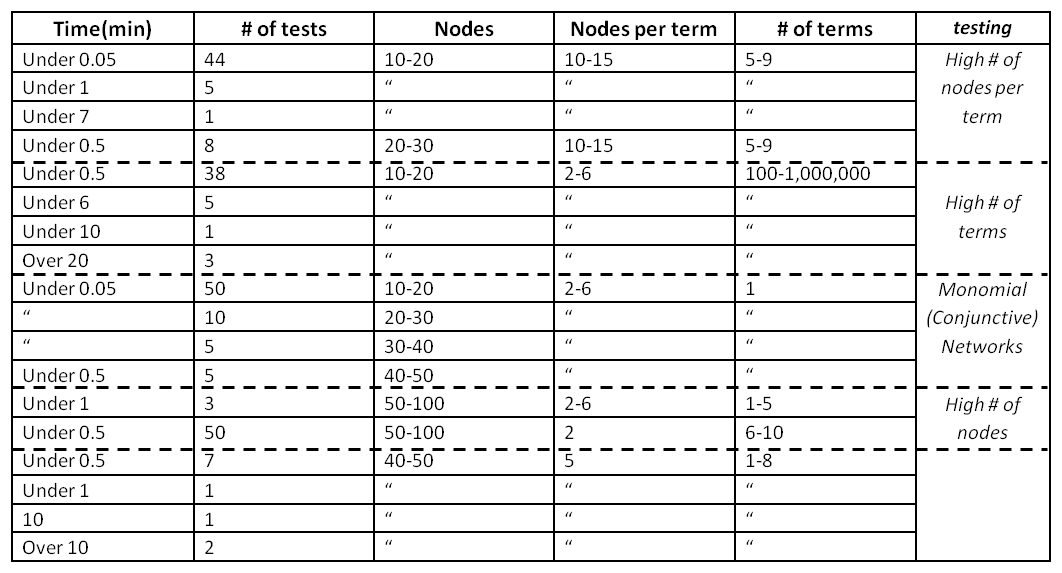
\includegraphics[scale=0.8]{benchmarkTable.png}
	\caption{Results of benchmark tests on Gr\"obner basis computations.}
	\label{tab:GBbenchmarks}
\end{table}
\end{comment}
91 percent of Gr\"obner basis computations completed in less than 30 seconds.  Note that in the tests for a `high \# of nodes per term' the range of variables per term is significantly more than would be expected in a real biological system.  We also tested the effect of analyzing functions with a lot of terms.  All benchmark tests were run on a 2.27 GHz processor.

The tests for `high \# of terms' is particularly significant for limit-cycle
computations as finding limit cycles depends on repeated compositions of the
functions, which destroys the sparse structure and results in functions with
many terms.  For the purpose of testing the software with Conjunctive
networks, benchmarks were also run on randomly generated monomial networks.
These tests demonstrate that the algorithms are particularly fast on systems of functions with terms involving few variables.  Based on the literature these constraints seem to be the norm for PDS which describe most biological systems.  Therefore, for most input systems, ADAM can compute fixed points and short limit cycles rather quickly.


In addition to theoretical testing, benchmark tests were done on 25 models from the GINsim repository, including two in excess of 50 nodes.  Fixed points and limit cycles up to length 20 were computed for all 25 models with 85 percent of computations finishing in less than a second and collectively all computations finishing in less than 30 minutes.
%% Do we want to keep the following sentences?
Note that although Figure ~\ref{fig:GINsimiFP} may give the impression that run time increase exponentially with the number of states this is not the case. The number of states along the x-axis does not increase linearly but rather explodes towards the right end of the axis accounting for the appearence of exponential growth.
\begin{comment}
\begin{figure}[h]
	\centering
	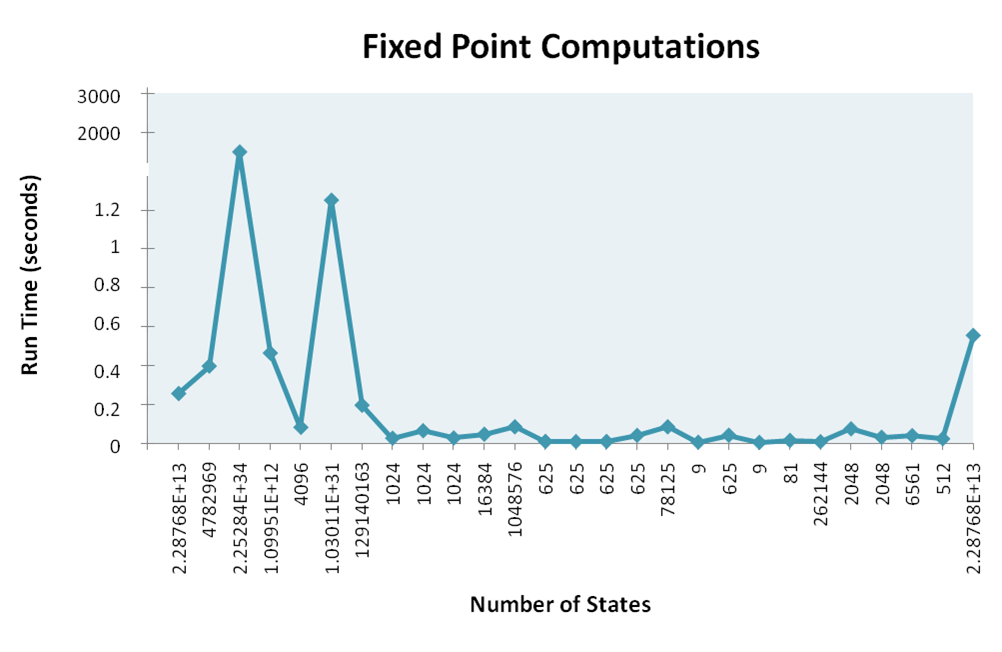
\includegraphics[scale=0.5]{GINsimFP.png}
	\caption{Plot representing run times for fixed point calculations done on 25
  Logical models.}
	\label{fig:GINsimFP}
\end{figure}
\end{comment}
A component is a set of states that have edges connecting to other states in the set. Put another way, if a state has no edges connecting to states in a component, then that state is not in the component. For instance, the above example, see Figure ~\ref{fig:SS}, has two components - one of size 3 and the other of size 5. The number of components and the component size are of significance because they inform how many different processes the system may be responsible for.

If a state only leads to itself, then it is a fixed point. In mathematical terms, this means $f(x) = x$. In Figure ~\ref{fig:SS}, $(000)$ would be a fixed point because it leads to itself. These are of interest because the researcher may then know what combination of on and off genes leads to a permanently fixed state, where no other changes in the states of the genes will produce a change in the system.  The continuous analog to a fixed point is a steady state.

A limit cycle is a set of points such that all other points in the component
lead to that set. Once a state in the limit cycle is reached only other states
in the limit cycle will be visited. In Figure ~\ref{fig:SS}, we have $010
\rightarrow 111$, $111 \rightarrow 011$, and $011 \rightarrow 010$, thus
$(010, 111, 011)$ is a limit cycle of length 3, or a 3-limit cycle. Note that
this limit cycle is also a component of the system.  We may be interested in
limit cycles and their length because they indicate recurring processes in the
cell cycle. For example, a 4-limit cycle in an embryonic cell could represent
the 4 different stages of the cell cycle. Typically a modeler expects small
limit cycles with large component sizes because that implies that small
perturbations in the environment will not greatly affect important cell
processes.


\begin{thebibliography}{5in}
\small
	\bibitem{Brown:1971} Brown W.S. (1971) On Euclid's Algorithm and the Computation of Polynomial Greatest Common Divisors. \textit{Journal of the ACM}.
  \bibitem{Leclerc:2008} Leclerc, Robert D. (2008) Survival of the Sparsest: Robust Gene Networks are Parsimonious. \textit{Ecology and Evolutionary Biology}.
	\bibitem{Remy:2005} Remy E., Ruet P., Thieffry D., (2005) Graphic Requirements for Multistability and Attractive Cycles in a Boolean Dynamical Framework. Advances in Applied Mathematics Volume 41, Issue 3, September 2008, Pages 335-350.
	\bibitem{Thomas:2001} Thomas R., (2001) Kaufman M., Multistationarity, The Basis of Cell Differentiation and Memory. I. Structural Conditions of Multistationarity and Other Nontrivial Behaviour. Chaos, Vol. 11, pp. 170-179.
	\bibitem{Ting:1999} Ting Chen, Hongyu L. He, George M. Church. (1999) Modeling Gene Expressions with Differential Equations. \textit{Genetics}.
\end{thebibliography}

\bibliographystyle{plain}
%\bibliographystyle{authordate1}
\bibliography{ADAM}
\end{document}
